\chapter{Referenciais Teóricos}
\label{cap:referenciais_teoricos}

% ---
\section{Aliquam vestibulum fringilla lorem}
% ---

\begin{figure}[!htb]
	\caption{Estrutura da molécula de DNA}
	\label{fig:estrutura_dna}
	\centering
	
\includegraphics[width=.3\textwidth]{estrutura_dna.eps} \\
	\begin{small}\textbf{Fonte: O Autor (2017)}\end{small}
\end{figure}

\lipsum[1]

\begin{grafico}[!htb]
	\caption{Estado do sequenciamento de genomas bacterianos}
	\label{grafico:gold_bacterial_sequencing_status}
	\centering
	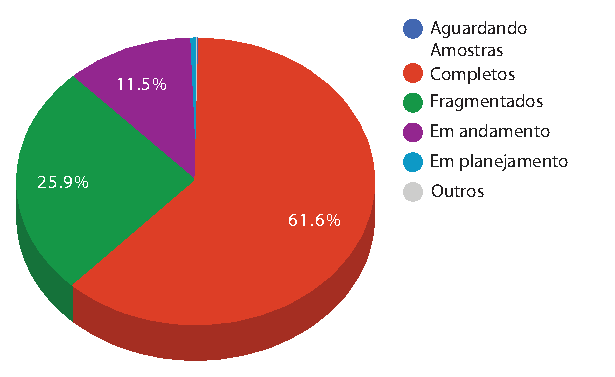
\includegraphics[width=.6\textwidth]{gold_bacterial_sequencing_status.eps} \\
	\begin{small}\textbf{Fonte: \citeonline{mukherjee2016}}\end{small}
\end{grafico}

\lipsum[2-3]

\chapter{Implementação}
\label{cap:implementacao}

\section{Algoritmo}

\begin{algorithm}[H]
   \SetAlgoLined
   \Entrada{$S,\eta, U$} 
   \Saida{Número esperado de nodos atingidos}
   \Inicio{
   $\sigma(S) = 0$ \\
    \Para{cada $u \in S$}{
   $\sigma(S)\leftarrow \sigma(S)+\textsc{Backtrack}(u,\eta,W,U)$\\
     }
   }
   \Retorna{$\sigma(S)$}
   \label{alg1}
   \caption{\textsc{Esperança}}
 \end{algorithm}
